% Capítulo revisado conforme a docs/thesis-revision-plan.md (2026-09-09).
% Archivo para incluir desde el documento principal de la tesis.
% Dependencias ya utilizadas por el original: array, float, pdflscape,
% tikz (arrows.meta), fontspec y las entradas bibliográficas conservadas.
% Compilar con XeLaTeX o LuaLaTeX. No contiene preámbulo ni bibliografía propia.
\chapter{Problema de Investigación}

\section{Fundamentación del problema de investigación}

La evolución de las redes de Service Provider (SP) ha transformado la forma en que estas se diseñan, operan y protegen. La demanda de servicios digitales, la proliferación de dispositivos conectados, la virtualización de funciones y la adopción de arquitecturas programables han incrementado la heterogeneidad de la infraestructura. En este contexto, los ataques de denegación de servicio (Denial of Service, DoS) y de denegación de servicio distribuido (Distributed Denial of Service, DDoS) constituyen amenazas para la disponibilidad y continuidad operacional.

Una red de SP puede reunir dominios enterprise, móvil, fijo y de interconexión o \textit{peering}, con fuentes de información, identidades y mecanismos de control diferentes. Cuando estas fuentes se analizan de manera independiente, resulta difícil establecer si varias observaciones corresponden al mismo tráfico en tránsito, a contribuciones de distintas fuentes o a incidentes simultáneos. También se dificulta determinar qué elemento puede actuar sobre cada fuente y comprobar si la respuesta produjo el efecto esperado.

La presente investigación aborda este problema mediante el diseño, implementación y evaluación de un \textbf{orquestador centralizado de análisis y decisión, con adquisición y ejecución distribuidas por dominio}. La centralización es lógica: las observaciones se integran para correlacionar incidentes y decidir un plan común, mientras que cada dominio aporta datos y ejecuta acciones mediante sus elementos de control. La mitigación distribuida no implica que la decisión sea descentralizada.

\subsection{Evolución de las redes de Service Provider}

Las redes de SP han incorporado progresivamente tecnologías que separan funciones de control, procesamiento y gestión de la infraestructura física. Software Defined Networking (SDN) permite programar políticas sobre elementos de red, mientras que Network Function Virtualization (NFV) facilita ejecutar funciones de telecomunicaciones sobre recursos computacionales de propósito general. Estas posibilidades ofrecen una base para instrumentar entornos experimentales y automatizar procedimientos de observación y respuesta.

En el dominio móvil, las arquitecturas de quinta generación y Open Radio Access Network (O-RAN) incorporan funciones e interfaces para observar y controlar la red de acceso radioeléctrico. El Near-Real-Time RAN Intelligent Controller (Near-RT RIC), sus aplicaciones xApps y los agentes de la RAN forman parte del camino de control contemplado en esta investigación. Las capacidades utilizables dependen, sin embargo, de las versiones y operaciones efectivamente soportadas por los componentes desplegados.

En el dominio fijo, las sesiones de abonado aportan un contexto diferente del disponible en un switch enterprise. Para el laboratorio se emplea BNGBlaster como instrumento de generación de tráfico y control experimental de sesiones. En enterprise se considera una infraestructura OpenFlow con Ryu y Open vSwitch (OVS). En peering se requiere observar tráfico en el borde y relacionarlo con interfaces y contexto de rutas BGP, además de disponer de un router capaz de aplicar la política seleccionada.

La convergencia de estos dominios crea una oportunidad de coordinación, pero no elimina sus diferencias. Una dirección IP, una sesión de abonado, un identificador de equipo de usuario (UE) o un puerto de switch no son selectores intercambiables. La investigación debe conservar su significado, su procedencia y su vigencia temporal para que una detección pueda traducirse en una acción sobre la entidad correcta.

\subsection{Evolución de las amenazas DoS/DDoS}

Los ataques de denegación de servicio buscan agotar recursos o degradar la prestación de un servicio. Los informes de amenazas incluidos en los antecedentes documentan ataques DDoS de gran volumen y motivan el estudio de mecanismos de protección \cite{Cloudflare_2024,Cloudflare_2025,NETSCOUT_2024}. Esa motivación no supone que el laboratorio reproduzca la escala de una red comercial ni que sus resultados puedan extrapolarse directamente a ella.

El alcance experimental obligatorio se delimita a \textbf{TCP SYN flood, UDP flood e ICMP flood}. El primer vector requiere evidencia de paquetes SYN y de su comportamiento respecto del establecimiento de conexiones; el volumen TCP agregado no basta para identificarlo. Los otros dos vectores se evaluarán a partir del protocolo, las tasas y los patrones temporales observados, contrastados con tráfico benigno. Se contemplan ataques simultáneos y combinaciones de estos vectores. Los ataques de aplicación, como HTTP flood, quedan fuera del alcance obligatorio y se consideran una extensión posterior.

Para esta investigación se distinguirán tres dimensiones. El \textit{vector} identifica el mecanismo del ataque; la \textit{distribución} distingue la contribución de una fuente de la de múltiples fuentes; y el \textit{alcance por origen} indica si estas pertenecen a uno o a varios dominios. En la matriz experimental, los casos DoS utilizarán una fuente de referencia y los DDoS utilizarán varias fuentes distintas y atribuibles. Esta es una convención operacional del laboratorio: DoS también designa la categoría general de denegación de servicio. La distribución geográfica no será un requisito, y el número de direcciones IP observadas no se equiparará al número de atacantes físicos demostrados.

Se considerará multidominio un incidente con contribuciones coincidentes de fuentes pertenecientes a dominios de origen distintos, relacionadas por el destino o servicio protegido y por su intervalo temporal. Por ejemplo, tráfico generado en el acceso móvil y observado nuevamente en el borde conserva un solo dominio de origen. Su doble observación no demuestra un ataque originado en móvil y peering, ni autoriza sumar dos veces su volumen. Asimismo, incidentes contra destinos distintos podrán tratarse como simultáneos sin agruparlos automáticamente en un único ataque.

La Figura \ref{fig:evolucion_red_amenaza} relaciona los cambios de infraestructura con los requisitos que motivan la propuesta. Representa una síntesis conceptual, no una correspondencia causal ni una cronología de resultados experimentales.

\begin{figure}[H]
    \centering
    \begin{tikzpicture}[
        box/.style={rectangle, rounded corners=3pt, draw=black, align=center,
            text width=3.8cm, minimum height=1.5cm, inner sep=5pt,
            font=\fontspec{Arial}\fontsize{10}{12}\selectfont},
        conn/.style={-{Latex[length=2mm]}, thick}
    ]
        \node[box] (r1) at (0,0) {Dominios heterogéneos\\e identidades propias};
        \node[box] (r2) at (4.8,0) {Interfaces programables\\y funciones virtualizadas};
        \node[box] (r3) at (9.6,0) {Servicios y tráfico\\entre dominios};
        \node[box] (t1) at (0,-2.7) {Observaciones parciales\\y calidad desigual};
        \node[box] (t2) at (4.8,-2.7) {TCP SYN, UDP e ICMP\\DoS y DDoS};
        \node[box] (t3) at (9.6,-2.7) {Correlación por origen\\y respuesta verificada};
        \draw[conn] (r1) -- (r2);
        \draw[conn] (r2) -- (r3);
        \draw[conn] (r1) -- (t1);
        \draw[conn] (r2) -- (t2);
        \draw[conn] (r3) -- (t3);
        \draw[conn] (t1) -- (t2);
        \draw[conn] (t2) -- (t3);
    \end{tikzpicture}
    \caption{Evolución de la infraestructura y requisitos de observación y respuesta considerados en el estudio.}
    \label{fig:evolucion_red_amenaza}
\end{figure}

\subsection{Problema de observabilidad fragmentada y necesidad de correlación multidominio}

La observabilidad requerida por el estudio combina flujos IP, estadísticas de red, eventos de sesión e información contextual de radio y enrutamiento. Estas fuentes describen fenómenos distintos. Las métricas Key Performance Measurements (KPM) de O-RAN aportan contexto de radio, pero no identifican por sí solas los tres vectores IP. Del mismo modo, el contexto de rutas BGP o de BGP Monitoring Protocol (BMP) no reemplaza la medición del tráfico que ingresa al borde.

Integrar observaciones requiere normalizar unidades, intervalos, calidad y procedencia. También exige distinguir el tiempo en que ocurrió el evento del tiempo en que se recibió, tratar retrasos y datos ausentes, y establecer un punto de medición autoritativo para contabilizar cada contribución. La suma de eventos recibidos durante un ciclo del controlador no constituye por sí sola una correlación temporal robusta.

La identidad debe resolverse para el intervalo observado. En móvil se requiere relacionar IP, sesión PDU, identidad de abonado y contexto RAN; en fijo, IP, sesión y VLAN; y en enterprise, fuente y ubicación en switch o puerto. Una asociación ambigua o vencida podrá conservarse como dato de calidad insuficiente, pero no habilitará una actuación individual que requiera una identidad inequívoca.

La correlación centralizada busca aprovechar estas observaciones para identificar aportes coincidentes y coordinar respuestas. Su utilidad deberá demostrarse mediante comparación experimental. La integración de fuentes o la presentación de un tablero, por sí solas, no acreditan detección correcta, control operativo ni mejora de disponibilidad.

\section{Formulación del problema de investigación}

El problema se sitúa en la integración verificable de observación, análisis y control entre cuatro dominios heterogéneos. La arquitectura debe determinar qué tráfico se ha observado, de dónde procede, qué evidencia respalda la detección, qué acción admite el dominio y cómo comprobar su aplicación, eficacia y retirada. La Tabla \ref{tab:observabilidad_actual_dominio} resume las fuentes y limitaciones que orientan la formulación; no pretende describir de forma universal los sistemas de todos los operadores.

\subsection{Problema general}

\begin{table}[H]
    \centering
    \renewcommand{\arraystretch}{1.25}
    \fontsize{10}{12}\selectfont
    \begin{tabular}{@{}>{\raggedright\arraybackslash}p{0.16\linewidth}
        >{\raggedright\arraybackslash}p{\dimexpr0.42\linewidth-2\tabcolsep\relax}
        >{\raggedright\arraybackslash}p{\dimexpr0.42\linewidth-2\tabcolsep\relax}@{}}
        \hline \textbf{Dominio} & \textbf{Fuentes consideradas} & \textbf{Limitación que debe resolverse} \\ \hline
        Móvil O-RAN & Flujos del plano de usuario, sesiones del core, asociaciones RAN y KPM. & Unir tráfico e identidad temporal; separar contexto de radio de evidencia del vector. \\ \hline
        Fijo & Flujos y estadísticas de BNGBlaster, IP, sesión y VLAN. & Distinguir flujos dentro de una sesión y medir el alcance del corte de acceso. \\ \hline
        Enterprise & Estadísticas OpenFlow, evidencia de flags y ubicación host/puerto. & Evitar duplicados y verificar selectores y reglas del switch. \\ \hline
        Peering BGP & Flujos de entrada al borde, interfaces y contexto de rutas. & Separar tránsito de origen y confirmar filtrado efectivo en el router. \\ \hline
    \end{tabular}
    \caption{Fuentes de observación y limitaciones de integración por dominio.}
    \label{tab:observabilidad_actual_dominio}
\end{table}

Cuando la observación y la respuesta se limitan al contexto local, puede perderse información sobre aportes coincidentes de otros dominios. No obstante, reunir todas las observaciones sin distinguir su origen o vigencia también puede producir errores: doble conteo, atribución a una sesión reasignada o una orden sobre un selector incorrecto. La investigación debe resolver ambos problemas y evaluar el costo y beneficio de la coordinación.

El problema general se formula de la siguiente manera:

\begin{quotation}
\textbf{\textit{¿Cómo diseñar, implementar y evaluar un orquestador centralizado que integre observaciones de los dominios móvil O-RAN, fijo con BNGBlaster, enterprise OpenFlow y peering BGP para detectar y correlacionar ataques DoS/DDoS TCP SYN, UDP e ICMP floods, incluidos escenarios multidominio, y coordinar mitigaciones específicas cuya aplicación y eficacia se verifiquen experimentalmente?}}
\end{quotation}

La detección temprana se tratará como una propiedad medible. Se registrará el tiempo entre el inicio conocido del ataque y su detección, junto con la evolución del servicio protegido. Cualquier afirmación de anticipación a una degradación deberá apoyarse en un criterio de degradación predefinido y en mediciones del servicio. No se deducirá el tiempo de mitigación a partir de la frecuencia del bucle de adquisición.

\subsection{Problemas específicos}

Los cinco problemas específicos se vinculan, respectivamente, con los objetivos OE1--OE5. La Tabla \ref{tab:problemas_especificos} mantiene esa correspondencia para que la operacionalización y la campaña experimental utilicen los mismos identificadores.

\begin{landscape}
\begin{table}[t]
    \centering
    \renewcommand{\arraystretch}{1.3}
    \fontsize{10}{12}\selectfont
    \begin{tabular}{@{}>{\raggedright\arraybackslash}p{0.06\linewidth}
        >{\raggedright\arraybackslash}p{\dimexpr0.22\linewidth-2\tabcolsep\relax}
        >{\raggedright\arraybackslash}p{\dimexpr0.47\linewidth-2\tabcolsep\relax}
        >{\raggedright\arraybackslash}p{\dimexpr0.25\linewidth-2\tabcolsep\relax}@{}}
        \hline \textbf{ID} & \textbf{Dimensión} & \textbf{Problema específico} & \textbf{Vinculación} \\ \hline
        PE1 & Fuentes, identidades y control & ¿Qué fuentes de observación, relaciones de identidad y capacidades efectivas de control están disponibles en cada uno de los cuatro dominios? & OE1: caracterización sustentada en inventario y pruebas de capacidad. \\ \hline
        PE2 & Normalización y correlación & ¿Cómo integrar observaciones con calidad desigual y correlacionarlas temporalmente y por identidad sin duplicar tráfico ni atribuirlo a una entidad incorrecta? & OE2: contratos, calidad, vigencia y deduplicación. \\ \hline
        PE3 & Detección y origen & ¿Cómo detectar los tres vectores, distinguir una fuente de múltiples fuentes y reconocer contribuciones de dominios de origen distintos, incluidos ataques simultáneos? & OE3: clasificación por vector, distribución y origen. \\ \hline
        PE4 & Ejecución y verificación & ¿Cómo traducir y ejecutar las mitigaciones soportadas por cada dominio y comprobar su aplicación, expiración y retirada, incluso ante fallos parciales? & OE4: ciclo de control y evidencia del resultado. \\ \hline
        PE5 & Evaluación comparativa & ¿Qué desempeño presenta la coordinación centralizada en detección, eficacia, impacto sobre tráfico legítimo y recuperación frente a respuestas independientes bajo condiciones equivalentes? & OE5: campaña reproducible, comparación e incertidumbre. \\ \hline
    \end{tabular}
    \caption{Problemas específicos y correspondencia con los objetivos.}
    \label{tab:problemas_especificos}
    \label{tab:ptoblemas_especificos}% Alias conservado por compatibilidad con la tesis.
\end{table}
\end{landscape}

La formulación no presupone superioridad de la coordinación centralizada en todos los escenarios. Esa relación se contrastará mediante indicadores y evidencia compatibles con cada problema, y no mediante la mera presencia de una funcionalidad en el software.

\section{Formulación de objetivos}

Los objetivos abarcan el diseño, la implementación y la evaluación de la solución. Su cumplimiento requiere integrar las fuentes y los elementos de control de los cuatro dominios, así como conservar evidencia suficiente para reconstruir las decisiones y sus efectos. El alcance corresponde a un entorno experimental controlado y no a una validación de despliegue productivo.

\subsection{Objetivo general}

\begin{quotation}
\textbf{\textit{Diseñar, implementar y evaluar un orquestador centralizado que integre telemetría e información de flujos de los dominios móvil O-RAN, fijo con BNGBlaster, enterprise OpenFlow y peering BGP, para detectar y correlacionar ataques DoS/DDoS TCP SYN, UDP e ICMP floods, incluidos escenarios multidominio, y coordinar acciones de mitigación específicas por dominio cuya aplicación y eficacia sean verificadas experimentalmente.}}
\end{quotation}

La aplicación de una acción y su eficacia se verificarán por separado. La primera exige comprobar el estado del elemento que ejecuta el control; la segunda exige medir el efecto sobre el tráfico malicioso y el servicio protegido. También se comprobarán el impacto sobre tráfico legítimo y la recuperación después de retirar la medida. Una respuesta de aceptación o un registro del orquestador no reemplaza estas verificaciones.

\subsection{Objetivos específicos}

La Tabla \ref{tab:objetivos_especificos} define los cinco objetivos y sus productos verificables. Estos enunciados constituyen la referencia para mantener la trazabilidad con los problemas específicos y con la posterior matriz de hipótesis, indicadores, experimentos y evidencia.

\begin{landscape}
\begin{table}[t]
    \centering
    \renewcommand{\arraystretch}{1.3}
    \fontsize{10}{12}\selectfont
    \begin{tabular}{@{}>{\raggedright\arraybackslash}p{0.06\linewidth}
        >{\raggedright\arraybackslash}p{\dimexpr0.42\linewidth-2\tabcolsep\relax}
        >{\raggedright\arraybackslash}p{\dimexpr0.27\linewidth-2\tabcolsep\relax}
        >{\raggedright\arraybackslash}p{\dimexpr0.25\linewidth-2\tabcolsep\relax}@{}}
        \hline \textbf{ID} & \textbf{Objetivo específico} & \textbf{Aspectos clave} & \textbf{Producto verificable} \\ \hline
        OE1 & Caracterizar fuentes de observación, identidades y capacidades efectivas de control de los cuatro dominios. & Versiones, puntos de medición, unidades, granularidad, selectores y operaciones soportadas. & Inventario y matriz de requerido, implementado, validado y evidencia; respuesta a PE1. \\ \hline
        OE2 & Diseñar e implementar contratos normalizados y correlación temporal y de identidad, con calidad y deduplicación de observaciones. & Tiempo de evento, red o VRF, vigencia de asociaciones, datos ausentes y puntos autoritativos. & Contratos y pruebas de reentrega, doble observación, retraso y reasignación; respuesta a PE2. \\ \hline
        OE3 & Implementar y evaluar detección por vector, distribución de fuentes y dominio de origen, incluyendo ataques simultáneos. & TCP SYN, UDP e ICMP; DoS/DDoS; origen distinto de tránsito; calibración separada. & Clasificación contrastada con verdad de referencia, matriz de confusión y falsos positivos; respuesta a PE3. \\ \hline
        OE4 & Implementar traducción y ejecución de mitigaciones por dominio, con confirmación, expiración, retirada y tratamiento de fallos parciales. & Capacidades e identidad válidas, ejecución asíncrona, idempotencia y reconciliación de estado. & Órdenes, respuestas, lectura posterior de estado y medición de efectos y retirada; respuesta a PE4. \\ \hline
        OE5 & Evaluar detección, eficacia, impacto sobre tráfico legítimo y recuperación mediante una campaña reproducible y comparativa. & Observación sin mitigación, respuesta local independiente y coordinación central; repeticiones e incertidumbre. & Resultados por ejecución, comparación de tiempos y servicio, dispersión y límites; respuesta a PE5. \\ \hline
    \end{tabular}
    \caption{Objetivos específicos, aspectos clave y productos verificables.}
    \label{tab:objetivos_especificos}
\end{table}
\end{landscape}

La implementación de peering y el control móvil mediante el RIC son requisitos del objetivo general. Su integración no se considerará una extensión opcional mientras se mantenga el alcance de cuatro dominios. Los ataques de aplicación y la ampliación a escala productiva quedan reservadas para trabajos posteriores.

\section{Justificación e importancia de la investigación}

La investigación se justifica por la necesidad de relacionar observaciones heterogéneas con decisiones y acciones comprobables. El aporte propuesto reside en los contratos de intercambio, la correlación temporal y de identidad, la deduplicación, la decisión centralizada, la traducción a controles por dominio y la verificación de eficacia. La disponibilidad y la resiliencia constituyen resultados por evaluar dentro del alcance experimental definido.

\subsection{Justificación científica}

El estudio permite examinar bajo condiciones controladas la relación entre visibilidad multidominio y respuesta coordinada. La pregunta científica no se limita a si es posible reunir métricas en una interfaz, sino a si la información integrada permite atribuir correctamente las contribuciones, detectar los vectores seleccionados y coordinar medidas que produzcan efectos medibles sobre el servicio.

La contribución se concreta en una representación común de observaciones e identidades con vigencia temporal y calidad explícita; un procedimiento para correlacionar aportes sin duplicar tráfico; y una evaluación del control que distingue intención, aceptación, aplicación y efecto. Los experimentos de doble observación, reasignación de IP y fallos parciales permitirán examinar condiciones en las que una integración incorrecta podría producir conclusiones engañosas.

La comparación con mecanismos independientes por dominio permitirá establecer en qué escenarios la coordinación resulta útil, indiferente o desfavorable. Si se mantiene una hipótesis de mejora, el tamaño de efecto relevante y el criterio estadístico deberán fijarse antes de la evaluación. La funcionalidad observada en el prototipo no se utilizará como prueba de una mejora significativa.

\subsection{Justificación tecnológica}

La heterogeneidad de los dominios exige una separación entre el significado de una intención de mitigación y la operación que puede ejecutarse localmente. Un contrato común deberá preservar el selector, la duración, la evidencia que sustenta la decisión y el resultado del control, mientras que el adaptador traducirá la intención a una capacidad comprobada. La Tabla \ref{tab:tecnologias_dominio} presenta los caminos del diseño objetivo.

\begin{table}[H]
    \centering
    \renewcommand{\arraystretch}{1.25}
    \fontsize{10}{12}\selectfont
    \begin{tabular}{@{}>{\raggedright\arraybackslash}p{0.18\linewidth}
        >{\raggedright\arraybackslash}p{\dimexpr0.82\linewidth-2\tabcolsep\relax}@{}}
        \hline \textbf{Dominio} & \textbf{Observación, control y comprobación previstos} \\ \hline
        Móvil O-RAN & Flujos antes de NAT en UPF, sesiones Open5GS, asociaciones de identidad RAN y KPM desde Gateway/RIC. Bridge/xApp hacia Near-RT RIC y operación E2SM-RC soportada en la RAN; respuesta, estado y efecto por UE. \\ \hline
        Fijo & Flujos medidos y estadísticas de BNGBlaster con asociación IP/sesión/VLAN. Control experimental de sesión, consulta del estado posterior y medición de tráfico y afectación de la sesión. \\ \hline
        Enterprise & Ryu, OVS y OpenFlow, con estadísticas y evidencia de flags. Regla de descarte o limitación de tasa soportada; consulta de reglas, errores y contadores, y comprobación de retirada. \\ \hline
        Peering BGP & Flujos de entrada al borde, interfaces y contexto de rutas. FlowSpec instalado por el router o mecanismo de gestión declarado; comprobación de instalación, contadores, efecto y retirada. \\ \hline
    \end{tabular}
    \caption{Caminos tecnológicos del diseño objetivo por dominio, sujetos a verificación.}
    \label{tab:tecnologias_dominio}
\end{table}

La existencia de un RIC no demuestra que la RAN admita la acción requerida; del mismo modo, anunciar una regla FlowSpec no acredita su instalación en el plano de datos. El diseño exige validar cada camino completo. En fijo, detener una sesión BNGBlaster constituye una actuación experimental sobre el acceso y puede interrumpir todo su tráfico, por lo que no se presentará como filtrado selectivo de un BNG de producción.

Los contratos y adaptadores favorecen la organización del software, pero una interfaz sin fuente de datos ni actuador operativo solo demuestra una abstracción. La extensibilidad operacional se acreditará al integrar un componente concreto, comprobar la semántica de sus datos y verificar las acciones y su retirada. Se conservará la distinción entre capacidades requeridas, implementadas y validadas.

\subsection{Justificación metodológica}

La metodología propuesta vincula cada resultado con una ejecución identificable y una verdad de referencia independiente. Se separarán los datos utilizados para calibrar de los empleados para evaluar. El escenario seleccionado en el generador no se proporcionará al detector como etiqueta de ataque, y las repeticiones conservarán configuraciones y condiciones comparables.

La campaña prevista comprende 24 configuraciones básicas (cuatro dominios, tres vectores y dos distribuciones DoS/DDoS), 18 configuraciones por parejas de dominios, tres configuraciones con los cuatro dominios y un escenario mixto adicional. Estas 46 configuraciones positivas se complementarán con líneas base benignas y pruebas de ambigüedad, fallo y retirada. Constituyen una cobertura propuesta antes de repeticiones; no representan resultados obtenidos ni todas las combinaciones posibles.

Para la comparación se ejecutarán tres condiciones: (A) observación sin mitigación, (B) detección y respuesta local independiente y (C) coordinación centralizada. Se mantendrán comparables el tráfico, los recursos y las capacidades de actuación. La Tabla \ref{tab:metodologia} resume los elementos que permiten evaluar el aporte de la coordinación.

\begin{table}[H]
    \centering
    \renewcommand{\arraystretch}{1.25}
    \fontsize{10}{12}\selectfont
    \begin{tabular}{@{}>{\raggedright\arraybackslash}p{0.29\linewidth}
        >{\raggedright\arraybackslash}p{\dimexpr0.71\linewidth-2\tabcolsep\relax}@{}}
        \hline \textbf{Componente} & \textbf{Procedimiento y evidencia} \\ \hline
        Diseño y referencia & Fuentes atribuibles, tráfico benigno, inicio y fin conocidos del ataque; configuraciones equivalentes en las tres condiciones. \\ \hline
        Calidad de detección & Precisión, sensibilidad, F1 y falsos positivos por vector y distribución; unidad de evaluación y asociación alerta/incidente definidas previamente. \\ \hline
        Tiempos de respuesta & Medir por separado detección, despacho, aplicación comprobada y tiempo hasta efecto; conservar sincronización e incertidumbre de reloj y sondeo. \\ \hline
        Eficacia y servicio & Tráfico malicioso en el punto protegido respecto de una referencia comparable; pérdida, latencia y rendimiento benignos antes, durante y después del control. \\ \hline
        Recuperación y fallos & Estado posterior a la retirada, restauración del servicio, rechazos, tiempos de espera agotados, reinicios y éxito parcial multidominio. \\ \hline
        Reproducibilidad & Identificador de ejecución, versiones y configuración, observaciones, decisiones, órdenes, respuestas y mediciones; repeticiones, dispersión e incertidumbre. \\ \hline
    \end{tabular}
    \caption{Componentes de la metodología experimental y evidencia requerida.}
    \label{tab:metodologia}
\end{table}

Las ventanas, los umbrales de detección y eficacia y el número definitivo de repeticiones se fijarán a partir del piloto y del criterio de evaluación. Las diez repeticiones por caso consideradas en el diseño constituyen una propuesta inicial de planificación, no una justificación estadística definitiva. Las ventanas solapadas no se contarán como ensayos independientes y los fallos o datos incompletos conservarán su causa e indicadores de calidad.

Se mantendrán separados tres estados del trabajo. La campaña de catorce subcasos y el simulador móvil corresponden al prototipo anterior y aportan evidencia preliminar de esa versión. El estado actual de migración incluye la retirada del simulador y la incorporación del contrato de observaciones y la correlación móvil al repositorio. El diseño objetivo exige integrar y validar los cuatro dominios. Los resultados históricos no se renombrarán como ensayos de la nueva plataforma; la actuación sobre el generador móvil no constituye validación de control E2SM-RC sobre la RAN.

\subsection{Justificación práctica}

La propuesta busca facilitar el análisis y la respuesta frente a incidentes que involucren fuentes de distintos dominios. Sus beneficios son expectativas sujetas a medición, como se explicita en la Tabla \ref{tab:beneficios_practicos}. La evaluación también debe identificar costos y límites, incluidos los efectos de acciones amplias, la pérdida de telemetría y la dependencia del orquestador central.

\begin{table}[H]
    \centering
    \renewcommand{\arraystretch}{1.25}
    \fontsize{10}{12}\selectfont
    \begin{tabular}{@{}>{\raggedright\arraybackslash}p{0.32\linewidth}
        >{\raggedright\arraybackslash}p{\dimexpr0.68\linewidth-2\tabcolsep\relax}@{}}
        \hline \textbf{Beneficio esperado} & \textbf{Condición para demostrarlo} \\ \hline
        Detección oportuna & Medir detección desde el inicio conocido y su relación con la degradación del servicio, sin perder precisión por agregar observaciones. \\ \hline
        Menor impacto del ataque & Comprobar reducción persistente de tráfico malicioso en el punto protegido respecto de una referencia comparable. \\ \hline
        Continuidad del servicio & Medir disponibilidad mediante sondas y un denominador temporal definido, además de pérdida, latencia y rendimiento del tráfico legítimo. \\ \hline
        Recuperación controlada & Verificar expiración o retirada, restauración del servicio y comportamiento ante fallos parciales o reinicios. \\ \hline
        Automatización trazable & Reconstruir la relación entre observación, decisión, orden y resultado; medir intervenciones si se afirma una reducción de trabajo manual. \\ \hline
        Visibilidad integrada & Acreditar fuentes operativas, datos recientes y atribución correcta en los cuatro dominios, además de la visualización. \\ \hline
    \end{tabular}
    \caption{Beneficios prácticos esperados y condiciones de verificación.}
    \label{tab:beneficios_practicos}
\end{table}

La utilidad para un operador dependerá de las capacidades de su infraestructura, de los límites de daño colateral y de la escala de operación. Por ello, la tesis reportará resultados del laboratorio con sus condiciones y restricciones, sin convertirlos automáticamente en garantías de funcionamiento en una red comercial.

\subsection{Importancia de la investigación}

La disponibilidad de las redes de SP sostiene servicios utilizados en actividades económicas, educativas y sociales. Estudiar mecanismos de protección coordinada resulta pertinente porque las decisiones sobre una fuente pueden afectar tanto al servicio protegido como al tráfico legítimo que comparte sesión, enlace o recurso.

La importancia del trabajo radica en ofrecer una implementación y un procedimiento experimental que permitan comprobar qué se observó, qué identidad se resolvió, qué medida se ejecutó y qué efecto produjo. Esta trazabilidad permite identificar tanto las ventajas de la coordinación como los casos en que una capacidad insuficiente o una observación ambigua impide actuar de manera adecuada.

\section{Viabilidad de la investigación}

La viabilidad se sustenta en el desarrollo existente y en la posibilidad de completar la integración mediante plataformas de laboratorio. Se considera \textbf{condicionada a la comprobación de las fuentes y capacidades de control pendientes}, especialmente en móvil y peering. La disponibilidad de software abierto no garantiza por sí sola interoperabilidad ni permite afirmar que el diseño completo ya esté implementado.

\subsection{Viabilidad técnica}

El repositorio dispone de componentes de adquisición y actuación para enterprise y fijo, así como de modelos, un adaptador de observaciones móviles y correlación temporal móvil. El simulador móvil anterior fue retirado. Estos componentes constituyen una base de migración, pero la entrada móvil requiere productores reales y el control mediante el RIC permanece pendiente de integración y verificación. El adaptador de peering no aporta todavía una adquisición operativa ni una validación de actuación en router.

La Tabla \ref{tab:viabilidad_tecnica} distingue esa base de trabajo de los requisitos pendientes. La existencia de código se considera evidencia de implementación de un componente, no evidencia suficiente de despliegue o validación de extremo a extremo.

\begin{table}[H]
    \centering
    \renewcommand{\arraystretch}{1.25}
    \fontsize{10}{12}\selectfont
    \begin{tabular}{@{}>{\raggedright\arraybackslash}p{0.17\linewidth}
        >{\raggedright\arraybackslash}p{\dimexpr0.36\linewidth-2\tabcolsep\relax}
        >{\raggedright\arraybackslash}p{\dimexpr0.47\linewidth-2\tabcolsep\relax}@{}}
        \hline \textbf{Componente} & \textbf{Base documentada} & \textbf{Dependencia y criterio pendiente} \\ \hline
        Enterprise & Ryu, colectores OpenFlow, mitigador y entorno Mininet/OVS. & Evidencia SYN, ausencia de doble conteo, reglas o limitadores soportados y lectura posterior de aplicación y retirada. \\ \hline
        Fijo & BNGBlaster y componentes de telemetría y control de sesiones. & Medir flujos y asociarlos temporalmente; confirmar tipo de sesión, efecto del corte y recuperación. \\ \hline
        Móvil: datos & Contrato y consumo de observaciones, asociaciones temporales y contexto KPM en el repositorio. & Exportadores UPF/Open5GS/RAN y lectura Gateway/RIC; unión de identidades y calidad verificadas con tráfico real del testbed. \\ \hline
        Móvil: control & Camino objetivo bridge/xApp, Near-RT RIC y agente RAN. & Seleccionar una operación RC soportada y demostrar efecto sobre la UE elegida usando otra UE como control. \\ \hline
        Peering & Interfaz de adaptación prevista; adquisición y control completos pendientes. & Elegir router, versión y exportador; instalar FlowSpec o política de gestión declarada, medir efecto y verificar retirada. \\ \hline
        Orquestación & Correlación, detección, decisión y despacho existentes como base de migración. & Normalización común, deduplicación entre observadores, ejecución persistente y estados que propaguen fallos y resultados reales. \\ \hline
    \end{tabular}
    \caption{Base técnica documentada y dependencias para completar la integración.}
    \label{tab:viabilidad_tecnica}
\end{table}

Antes de la campaña se registrarán versiones, configuración, recursos de cómputo, distribución en máquinas virtuales o contenedores, interfaces y puntos de medición. Se comprobarán relojes, rutas, ubicación de la medición móvil antes de NAT y capacidad de los exportadores para proporcionar contadores y evidencia de protocolos. No se asumirán recursos físicos, rendimiento ni versiones que no figuren en el inventario comprobado.

El hito móvil exige una orden que atraviese el RIC, alcance el agente RAN y produzca un efecto comprobado sobre la UE seleccionada. Si la operación no está soportada, será necesario desarrollar o adaptar el control, o seleccionar un componente compatible; filtrar en UPF podrá servir como contingencia, pero no satisfará por sí solo el requisito de control vía RIC. En peering se exigirá un router que aplique la política en el plano de datos; un emisor de anuncios o un tablero disponible no completan ese requisito.

Para fijo se declarará si las sesiones evaluadas son IPoE, PPPoE o ambas, según la configuración realmente ejecutada. Cualquier participación de DHCP o de reglas adicionales de filtrado se identificará por separado. En todos los dominios, la ausencia de telemetría se tratará como pérdida de observación y no como prueba de recuperación.

\subsection{Viabilidad económica}

La estrategia económica consiste en reutilizar recursos de cómputo y componentes abiertos cuando resulten compatibles con los requisitos del experimento. Esto puede reducir el gasto en licencias, pero no elimina los costos de integración, almacenamiento de evidencia, operación del laboratorio ni posibles extensiones de control. La Tabla \ref{tab:componentes_tecnologicos} identifica los rubros que deben presupuestarse sin atribuir costos o licencias a versiones aún no seleccionadas.

\begin{table}[H]
    \centering
    \renewcommand{\arraystretch}{1.25}
    \fontsize{10}{12}\selectfont
    \begin{tabular}{@{}>{\raggedright\arraybackslash}p{0.34\linewidth}
        >{\raggedright\arraybackslash}p{\dimexpr0.66\linewidth-2\tabcolsep\relax}@{}}
        \hline \textbf{Componente} & \textbf{Criterio económico y dependencia} \\ \hline
        Ryu, OVS y Mininet & Reutilizar la base enterprise y verificar licencias y versiones del inventario. \\ \hline
        BNGBlaster y medición fija & Reutilizar el entorno existente; prever instrumentación de flujos y almacenamiento de capturas. \\ \hline
        Open5GS, RAN, RIC y xApps & Presupuestar integración de exportadores, pruebas de identidad y eventual desarrollo de control RC. \\ \hline
        Router y exportador de peering & Evaluar disponibilidad, licencia y costo del componente compatible con la política de filtrado requerida. \\ \hline
        Cómputo y almacenamiento & Estimar CPU, memoria, disco, retención de evidencia y tiempo de uso con mediciones del piloto. \\ \hline
    \end{tabular}
    \caption{Componentes y dependencias para la estimación económica.}
    \label{tab:componentes_tecnologicos}
\end{table}

La infraestructura se organizará conforme a la Tabla \ref{tab:opciones_infraestructura}. Esta describe usos y comprobaciones necesarias; no constituye una certificación de equipos disponibles ni un presupuesto cerrado.

\begin{table}[H]
    \centering
    \renewcommand{\arraystretch}{1.25}
    \fontsize{10}{12}\selectfont
    \begin{tabular}{@{}>{\raggedright\arraybackslash}p{0.34\linewidth}
        >{\raggedright\arraybackslash}p{\dimexpr0.66\linewidth-2\tabcolsep\relax}@{}}
        \hline \textbf{Recurso} & \textbf{Uso y comprobación necesaria} \\ \hline
        Equipo de desarrollo & Edición, pruebas de componentes y análisis; registrar capacidad y evitar interferencia con ensayos medidos. \\ \hline
        Máquinas virtuales o servidores de laboratorio & Alojar orquestador, core, RAN/RIC y router según el despliegue real; documentar límites de VM, interfaces y asignación de recursos. \\ \hline
        Emulación y contenedores & Mantener Mininet/OVS donde se utilice y empaquetar componentes compatibles; comprobar conectividad con los demás dominios. \\ \hline
        Almacenamiento y medición & Conservar configuraciones, registros, capturas y resultados; dimensionar retención y sondas del servicio protegido. \\ \hline
    \end{tabular}
    \caption{Recursos de infraestructura y comprobaciones para el despliegue experimental.}
    \label{tab:opciones_infraestructura}
\end{table}

La viabilidad económica se confirmará al cerrar el inventario y estimar la duración de las repeticiones. El uso de emulación reduce algunas necesidades de equipamiento, pero no sustituye la integración móvil ni la capacidad efectiva del router que exige el diseño.

\subsection{Viabilidad operativa}

El desarrollo incremental permite separar la validación de datos, identidad y actuación antes de integrar el sistema completo. La Tabla \ref{tab:conocimientos_requeridos} organiza las capacidades necesarias; su enumeración expresa necesidades operativas, no una certificación de disponibilidad de personal especializado.

\begin{table}[H]
    \centering
    \renewcommand{\arraystretch}{1.25}
    \fontsize{10}{12}\selectfont
    \begin{tabular}{@{}>{\raggedright\arraybackslash}p{0.30\linewidth}
        >{\raggedright\arraybackslash}p{\dimexpr0.70\linewidth-2\tabcolsep\relax}@{}}
        \hline \textbf{Área} & \textbf{Capacidad requerida} \\ \hline
        Redes y telecomunicaciones & Operar OpenFlow, sesiones de acceso, core móvil, RAN/RIC y router BGP; identificar puntos de observación y control. \\ \hline
        Desarrollo e integración & Implementar exportadores, contratos, asociaciones temporales, deduplicación, traducción de acciones y reconciliación de estado. \\ \hline
        Experimentación & Generar tráfico controlado, sincronizar relojes, verificar efectos y retirada, conservar verdad de referencia y analizar incertidumbre. \\ \hline
        Operación del laboratorio & Aislar escenarios, documentar arranque y recuperación y proteger registros que contengan IP, SUPI u otras identidades. \\ \hline
    \end{tabular}
    \caption{Áreas de conocimiento y capacidades operativas requeridas.}
    \label{tab:conocimientos_requeridos}
\end{table}

Se prepararán procedimientos de arranque, comprobación de conectividad, ejecución, recolección de evidencia y limpieza. Cada ensayo identificará sus fuentes, configuración y acciones, y finalizará con una comprobación de retirada. Las condiciones sin ataque se evaluarán por la ausencia de mitigaciones indebidas; no se contarán como ataques mitigados.

La aceptación de los componentes exigirá que un rechazo, un tiempo de espera agotado o una operación no soportada no se registren como éxito. Los planes multidominio conservarán los resultados individuales y reflejarán fallos parciales. Esta disciplina permite continuar la integración sin confundir una respuesta de software con un efecto real sobre la red.

\subsection{Viabilidad temporal}

La planificación considera integración, calibración, repetición experimental y análisis. Los hitos de control móvil y peering son dependencias de la validación completa y deben investigarse al inicio, porque pueden requerir cambios en el RIC, la RAN o el router. La Tabla \ref{tab:fases_ejecucion} establece actividades y criterios de salida.

\begin{table}[H]
    \centering
    \renewcommand{\arraystretch}{1.2}
    \fontsize{10}{12}\selectfont
    \begin{tabular}{@{}>{\raggedright\arraybackslash}p{0.10\linewidth}
        >{\raggedright\arraybackslash}p{\dimexpr0.39\linewidth-2\tabcolsep\relax}
        >{\raggedright\arraybackslash}p{\dimexpr0.51\linewidth-2\tabcolsep\relax}@{}}
        \hline \textbf{Fase} & \textbf{Actividad} & \textbf{Criterio de salida} \\ \hline
        I & Revisión, alcance e inventario & Problemas y objetivos alineados; recursos y capacidades pendientes identificados. \\ \hline
        II & Contratos y estados de control & Unidades, identidad, evidencia y fallos definidos; resultados del adaptador propagados. \\ \hline
        III & Integración enterprise y fijo & Datos y control comprobados; granularidad y tipo de sesión declarados. \\ \hline
        IV & Adquisición e identidad móvil & Flujos, sesiones y contexto RAN/KPM reales con asociación temporal validada. \\ \hline
        V & Implementación de peering & Exportación operativa y política instalada, medida y retirada por el router. \\ \hline
        VI & Implementación de control móvil & Acción vía RIC/RAN comprobada sobre una UE y contraste con otra UE. \\ \hline
        VII & Correlación y detección & Tres vectores, distribución y origen; pruebas de retraso, identidad y doble observación. \\ \hline
        VIII & Ejecución y recuperación & Planes por dominio, expiración, retirada, reinicio y fallos parciales verificados. \\ \hline
        IX & Piloto y calibración & Recursos, umbrales, criterios y repeticiones fijados antes de evaluar. \\ \hline
        X & Campaña comparativa repetida & Configuraciones positivas, negativos y fallos en condiciones comparables, con evidencia por ejecución. \\ \hline
        XI & Análisis y contraste & Métricas, dispersión, incertidumbre y contraste de hipótesis con evidencia correspondiente. \\ \hline
        XII & Redacción y sustentación & Resultados históricos separados de los nuevos; conclusiones limitadas a lo medido. \\ \hline
    \end{tabular}
    \caption{Fases de ejecución e hitos de aceptación de la investigación.}
    \label{tab:fases_ejecucion}
\end{table}

La Figura \ref{fig:cronograma_fases} utiliza dieciséis periodos relativos. Su duración se calendarizará después de comprobar recursos y estimar el esfuerzo del piloto. Las barras indican intervalos de trabajo previstos y no porcentajes de avance. Las fases V y VI comienzan con la comprobación de capacidades; la fase IX podrá preparar instrumentos antes, pero su cierre requerirá completar las integraciones y el control de las fases III--VIII.

\begin{figure}[H]
    \centering
    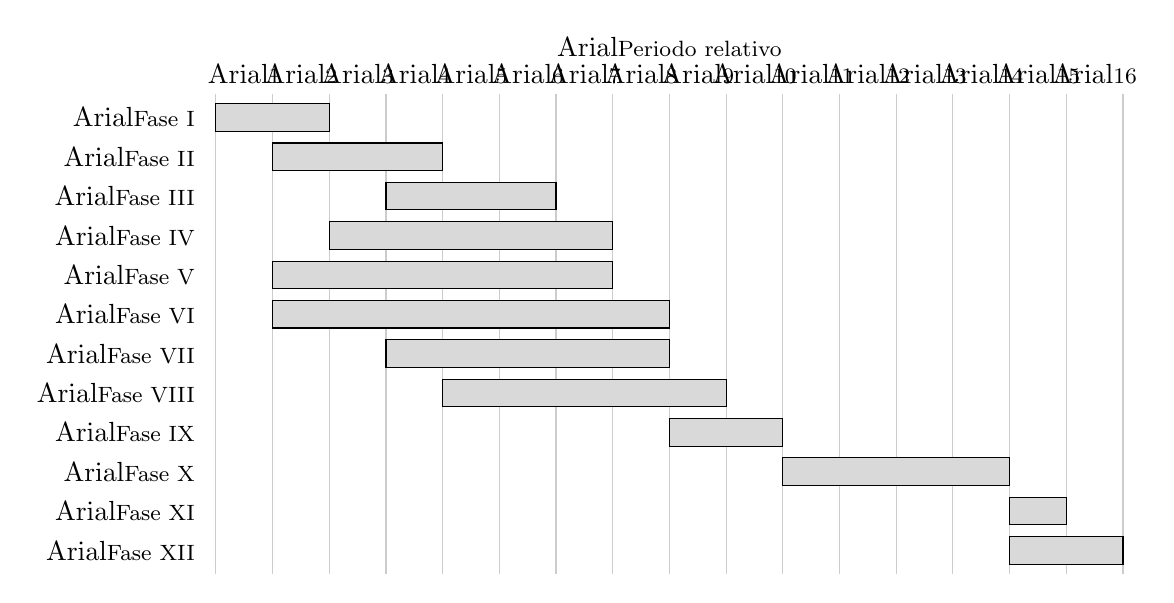
\begin{tikzpicture}[
        every node/.style={font=\fontspec{Arial}\fontsize{8}{10}\selectfont, text=black},
        bar/.style={draw=black, fill=black!15},
        xscale=0.72, yscale=0.5
    ]
        \foreach \p in {0,...,16} {
            \draw[gray!40] (\p,0.1) -- (\p,-12.1);
        }
        \foreach \p [count=\i from 0] in {1,...,16} {
            \node at (\i+0.5,0.6) {\p};
        }
        \node at (8,1.3) {Periodo relativo};
        \node[anchor=east] at (-0.2,-0.5)  {Fase I};    \draw[bar] (0,-0.85) rectangle (2,-0.15);
        \node[anchor=east] at (-0.2,-1.5)  {Fase II};   \draw[bar] (1,-1.85) rectangle (4,-1.15);
        \node[anchor=east] at (-0.2,-2.5)  {Fase III};  \draw[bar] (3,-2.85) rectangle (6,-2.15);
        \node[anchor=east] at (-0.2,-3.5)  {Fase IV};   \draw[bar] (2,-3.85) rectangle (7,-3.15);
        \node[anchor=east] at (-0.2,-4.5)  {Fase V};    \draw[bar] (1,-4.85) rectangle (7,-4.15);
        \node[anchor=east] at (-0.2,-5.5)  {Fase VI};   \draw[bar] (1,-5.85) rectangle (8,-5.15);
        \node[anchor=east] at (-0.2,-6.5)  {Fase VII};  \draw[bar] (3,-6.85) rectangle (8,-6.15);
        \node[anchor=east] at (-0.2,-7.5)  {Fase VIII}; \draw[bar] (4,-7.85) rectangle (9,-7.15);
        \node[anchor=east] at (-0.2,-8.5)  {Fase IX};   \draw[bar] (8,-8.85) rectangle (10,-8.15);
        \node[anchor=east] at (-0.2,-9.5)  {Fase X};    \draw[bar] (10,-9.85) rectangle (14,-9.15);
        \node[anchor=east] at (-0.2,-10.5) {Fase XI};   \draw[bar] (14,-10.85) rectangle (15,-10.15);
        \node[anchor=east] at (-0.2,-11.5) {Fase XII};  \draw[bar] (14,-11.85) rectangle (16,-11.15);
    \end{tikzpicture}
    \caption{Cronograma referencial de integración, calibración y evaluación en periodos relativos no calendarizados.}
    \label{fig:cronograma_fases}
\end{figure}

La fase X debe reservar tiempo para ataques, restablecimiento de líneas base, comprobación de retirada, repeticiones y conservación de fallos. Como referencia de carga, ejecutar las 46 configuraciones positivas en tres condiciones con diez repeticiones supondría 1380 ejecuciones positivas, además de los casos negativos y de fallo. Esta cifra es una estimación de planificación sujeta al diseño definitivo, no un número de experimentos realizados.

La ejecución paralela de actividades se limitará a tareas cuyas dependencias y recursos lo permitan. Los ensayos comparativos no compartirán recursos de manera que alteren las condiciones sin registrarlo. El análisis final se realizará sobre la campaña concluida, y los retrasos de control móvil o peering obligarán a revisar el calendario; no se declarará completado el alcance por sustituirlos con interfaces vacías o resultados del prototipo anterior.

En consecuencia, existen bases para avanzar incrementalmente, pero la viabilidad completa deberá confirmarse al superar los hitos de instrumentación y control, cerrar el inventario y completar el piloto. La planificación permitirá documentar tanto los resultados satisfactorios como las limitaciones de integración, manteniendo la separación entre el diseño propuesto y las capacidades efectivamente demostradas.
